%%%%%%%%%%%%%%%%%%%%%%%%%%%%%%%%%%%%%%%%%
% Beamer Presentation
% LaTeX Template
% Version 1.0 (10/11/12)
%
% This template has been downloaded from:
% http://www.LaTeXTemplates.com
%
% License:
% CC BY-NC-SA 3.0 (http://creativecommons.org/licenses/by-nc-sa/3.0/)
%
%%%%%%%%%%%%%%%%%%%%%%%%%%%%%%%%%%%%%%%%%

%----------------------------------------------------------------------------------------
%	PACKAGES AND THEMES
%----------------------------------------------------------------------------------------

\documentclass{beamer}

\mode<presentation> {

% The Beamer class comes with a number of default slide themes
% which change the colors and layouts of slides. Below this is a list
% of all the themes, uncomment each in turn to see what they look like.

%\usetheme{default}
%\usetheme{AnnArbor}
%\usetheme{Antibes}
%\usetheme{Bergen}
%\usetheme{Berkeley}
%\usetheme{Berlin}
%\usetheme{Boadilla}
%\usetheme{CambridgeUS}
%\usetheme{Copenhagen}
%\usetheme{Darmstadt}
%\usetheme{Dresden}
\usetheme{Frankfurt}
%\usetheme{Goettingen}
%\usetheme{Hannover}
%\usetheme{Ilmenau}
%\usetheme{JuanLesPins}
%\usetheme{Luebeck}
%\usetheme{Madrid}
%\usetheme{Malmoe}
%\usetheme{Marburg}
%\usetheme{Montpellier}
%\usetheme{PaloAlto}
%\usetheme{Pittsburgh}
%\usetheme{Rochester}
%\usetheme{Singapore}
%\usetheme{Szeged}
%\usetheme{Warsaw}

% As well as themes, the Beamer class has a number of color themes
% for any slide theme. Uncomment each of these in turn to see how it
% changes the colors of your current slide theme.

%\usecolortheme{albatross}
%\usecolortheme{beaver}
%\usecolortheme{beetle}
\usecolortheme{crane}
%\usecolortheme{dolphin}
%\usecolortheme{dove}
%\usecolortheme{fly}
%\usecolortheme{lily}
%\usecolortheme{orchid}
%\usecolortheme{rose}
%\usecolortheme{seagull}
%\usecolortheme{seahorse}
%\usecolortheme{whale}
%\usecolortheme{wolverine}

%\setbeamertemplate{footline} % To remove the footer line in all slides uncomment this line
%\setbeamertemplate{footline}[page number] % To replace the footer line in all slides with a simple slide count uncomment this line

%\setbeamertemplate{navigation symbols}{} % To remove the navigation symbols from the bottom of all slides uncomment this line
}

\usepackage{graphicx} % Allows including images
\usepackage{booktabs} % Allows the use of \toprule, \midrule and \bottomrule in tables

%----------------------------------------------------------------------------------------
%	TITLE PAGE
%----------------------------------------------------------------------------------------

\title[Rudiments of N. C.]{Rudiments of Neural Cryptography} % The short title appears at the bottom of every slide, the full title is only on the title page

\author{Francesco Moraglio} % Your name
\institute[UniTO] % Your institution as it will appear on the bottom of every slide, may be shorthand to save space
{
University of Torino \\ % Your institution for the title page
\medskip
%\textit{john@smith.com} % Your email address
}
\date{21/07/2020} % Date, can be changed to a custom date

\begin{document}

\begin{frame}
\titlepage % Print the title page as the first slide
\end{frame}

\begin{frame}
\frametitle{Overview} % Table of contents slide, comment this block out to remove it
\tableofcontents % Throughout your presentation, if you choose to use \section{} and \subsection{} commands, these will automatically be printed on this slide as an overview of your presentation
\end{frame}

%----------------------------------------------------------------------------------------
%	PRESENTATION SLIDES
%----------------------------------------------------------------------------------------

%------------------------------------------------
\section{Neural Networks} % Sections can be created in order to organize your presentation into discrete blocks, all sections and subsections are automatically printed in the table of contents as an overview of the talk
%------------------------------------------------



\begin{frame}
\frametitle{Neural Networks}
Artificial Neural Networks (ANNs) are models of computation based loosely on the way in which the brain is believed to work. A biological neural network consists of interconnected nerve cells, whose bodies are where neural processing takes place. \\
\begin{figure}
\centering
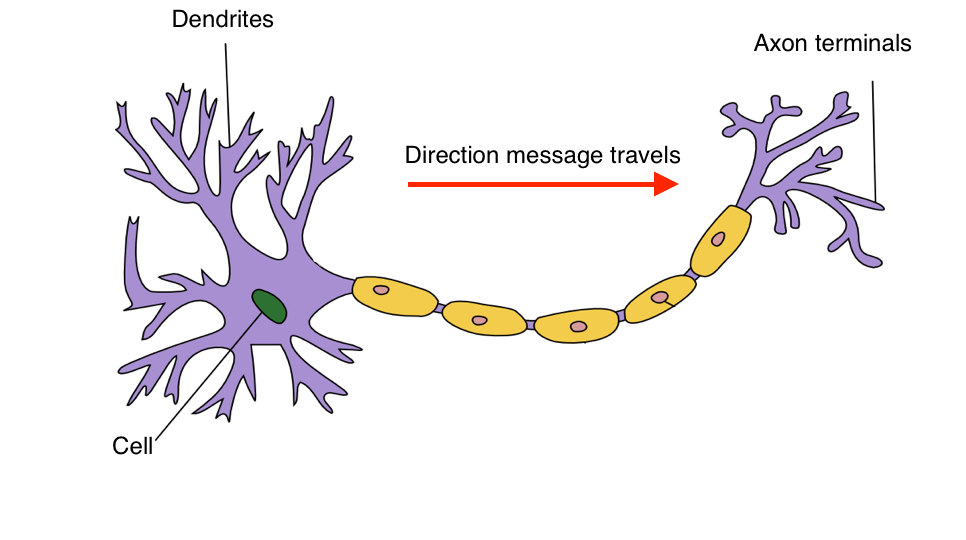
\includegraphics[width = \textwidth]{"pictures/neuron.png"}
\end{figure}

\end{frame}

%------------------------------------------------

\begin{frame}
\frametitle{Artificial Neural Networks}
Interconnections between cells are not all equally weighted: this is the key feature modeled by ANNs. Their theoretical principles were firstly formulated in the forties. Among them, a fundamental, widely applied learning principle is the following.
\begin{block}{Hebbian Learning Law}
When an axon of cell $A$ is near-enough to excite cell $B$ and when it repeatedly and persistently takes part in firing it, then some growth process
or metabolic change takes place in one or both these cells such that the efficiency of cell $A$ is increased.
\end{block}
\end{frame}

%------------------------------------------------

\begin{frame}
\frametitle{Perceptron: 1}
The first complete neural model is called Perceptron and appeared in the late fifties. It serves as a building block to most later models.
\begin{figure}
\centering
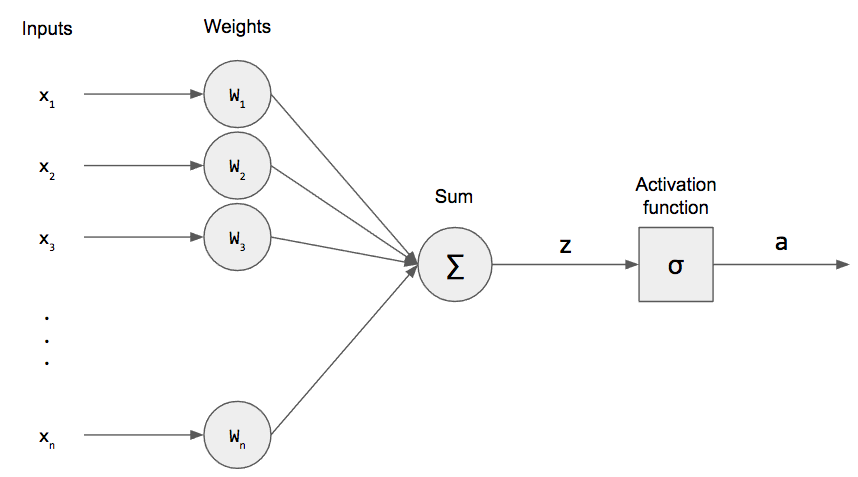
\includegraphics[width = 0.85\textwidth]{"pictures/perceptron.png"}
\end{figure}
\end{frame}
%------------------------------------------------

\begin{frame}
\frametitle{Perceptron: 2}
The input/output relations of the Perceptron are defined to be
\begin{align*}
z = \sum_{i}w_i x_i \quad &\text{(summation output)} \\
y = f_N(z) \quad &\text{(cell output)}, 
\end{align*}
where $w_i$ is the (adjustable) weight at input $x_i$. Function $f_N$ is nonlinear and is called activation. Typical activation functions used in ANNs include
\begin{itemize}
\item sigmoid function;
\item hyperbolic tangent;
\item Heaviside step function.
\end{itemize}
\end{frame}

%----------------------------------------------
\begin{frame}
\frametitle{Training}
The training of an ANN is the procedure of adjusting its weight. This task can be performed with several techniques. For the simplest architectures, we recall
\begin{itemize}
\item \textbf{Least Mean Square}. Minimizes the (approximated) square expectation of the error over all training sets. It is simple, but it is suitable only for bipolar perceptrons and may lead to inaccurate results.
\item \textbf{Gradient Descent}. Attempts to provide weight-setting estimates from one training set to the next.
\end{itemize}
\end{frame}
%----------------------------------------------

\begin{frame}
\begin{figure}
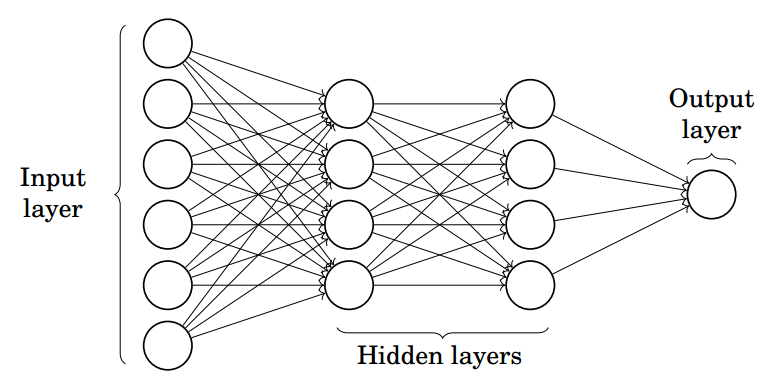
\includegraphics[height = 0.4\textheight]{"pictures/multilayer-perceptron.png"}
\end{figure}
More advanced algorithms were required to set weights of Multi-Layer Perceptrons (MLPs), whose computational capabilities are sensitively higher than those of single-layer NNs. 
\begin{itemize}
\item \textbf{Back Propagation (BP)} was developed with this specific purpose. It is an extension of the Gradient Descent method, that "propagates" from the last layer back to the first one, iterating over a pre-fixed set of training vectors.
\end{itemize}
\end{frame}

%--------------------------------------------
\begin{frame}
\frametitle{Adam}
\textbf{Adam}, a recent method for stochastic optimization, revealed itself to be a powerful tool for the training of most modern NN architectures. Let $f(\theta)$ be a noisy objective function; we are interested in minimizing $\mathbb{E}\left[f(\theta)\right]$.
\begin{itemize}
\item Consider $g_t = \nabla_{\theta}f_t(\theta)$, the gradient evaluated at time step $t$.
\item Adam works by updating exponential moving averages of the gradient and of the squared gradient.
\item Exponential decay rates of such moving averages are controlled by hyperparameters.
\end{itemize}
Name "Adam" is derived from "adaptive moment estimation".
\end{frame}



%------------------------------------------------
\section{Genetic Algorithms}
%------------------------------------------------

\begin{frame}
\frametitle{Genetic Algorithms: 1}
Genetic Algorithms (GAs) were invented by John Holland in the 1960s and can
be considered a key building block of artificial intelligence. These are stochastic search algorithms that can generate  
"sufficiently good" solutions to an optimization problem. Nowdays GAs are widely employed
in applied science and, in neural cryptography, they can be used to
\begin{itemize}
\item optimize network architectures involved in communication;
\item perform effective cryptanalitic attacks.
\end{itemize}
\end{frame}

%------------------------------------------------
\begin{frame}
\frametitle{Genetic Algorithms: 2}
\begin{columns}[c]
\column{.5\textwidth}
\begin{figure}[h]
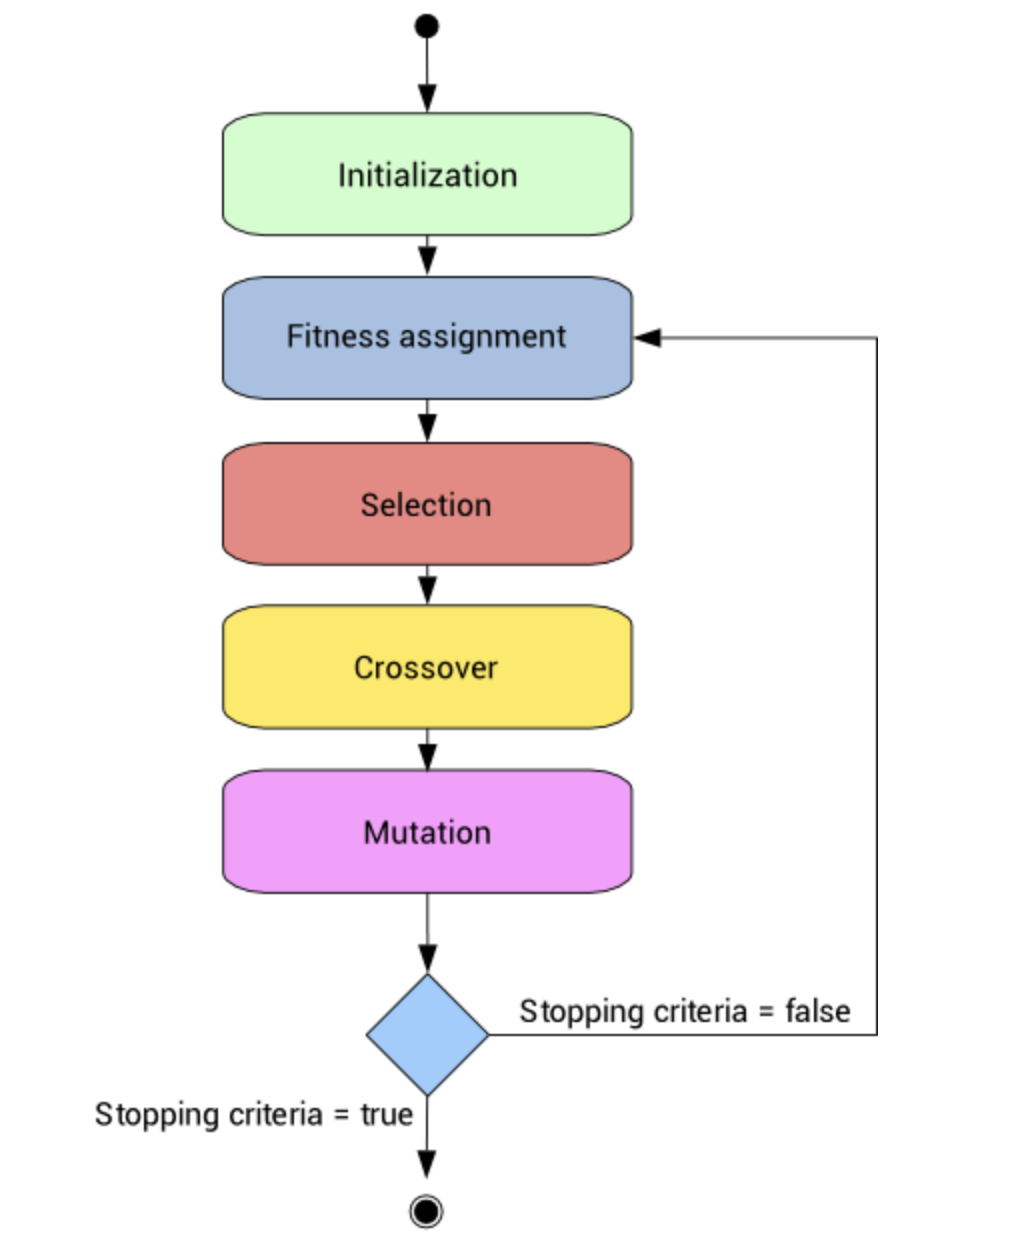
\includegraphics[width = \textwidth]{"pictures/genetic_algo.png"}
\end{figure}
\column{.65\textwidth}
\begin{itemize}
\item The GA is a method for evolving from a population of "chromosomes" (elements of a solution space) to a new population
by using an imitation of natural selection together with the genetic-inspired operators of crossover and mutation.
\item The main theoretical result on the behavior of GAs is known as Holland Theorem. It implies that the best "building blocks" of the solutions propagate exponentially over time in the population.
\end{itemize}


\end{columns}
\end{frame}


%------------------------------------------------
\section{Neural Cryptography}
\begin{frame} % Need to use the fragile option when verbatim is used in the slide
\frametitle{Neural Cryptography}
\begin{itemize}
\item From the nineties on, researchers have made attempts at combining the features of neural networks with cryptography: this field is commonly known as neurocryptography.
\item One of the first attempts can be found in \cite{volna}. In this work, the author builds a symmetric cryptosystem by making use of neural networks, whose parameters constitute the key of the cipher.
\item GAs are used for the optimization of the designed NN topology. Adaptation of the best found network architecture is then finished with BP.
\end{itemize}
\end{frame}
%-----------------------------------------------
\begin{frame}
\frametitle{The NNs of Volná}
The GA of Volná evolves the architecture of feedforward NNs whose weights are initialized as follows. For every existing connection, three digits are generated and weights are computed as 
\begin{align*}
w_{ij,kl} = \eta[e_2(e_1 2^1 + e_0 2^0)]; \quad i,k\in\{1,\dots,L\}, \\
  j\in\{1,\dots, n_i\}, \\
  l \in\{1, \dots, n_k\},
\end{align*}
where $w_{ij,kl} = w(x_{ij}, x_{kl})$ is the weight value between the $j$-th unit in the $i$-th layer and the $l$-th unit in the $k$-th layer and
\begin{align*}
    \eta &= \text{learning parameter;} \quad \eta \in (0,1)\\
    e_0, e_1 &= \text{random digits} \\
  	e_2 &= \text{sign bit}.
\end{align*}
\end{frame}

%-----------------------------------------------
\begin{frame}
\frametitle{KKK Key Exchange Protocol}
The first complete cryptosystem based on neural network is known in literature as KKK, from the surnames of its inventors \cite{kanter}. \\
This protocol is based on the synchronization of the weights of two tree parity machines, that represent the participants.
\begin{figure}
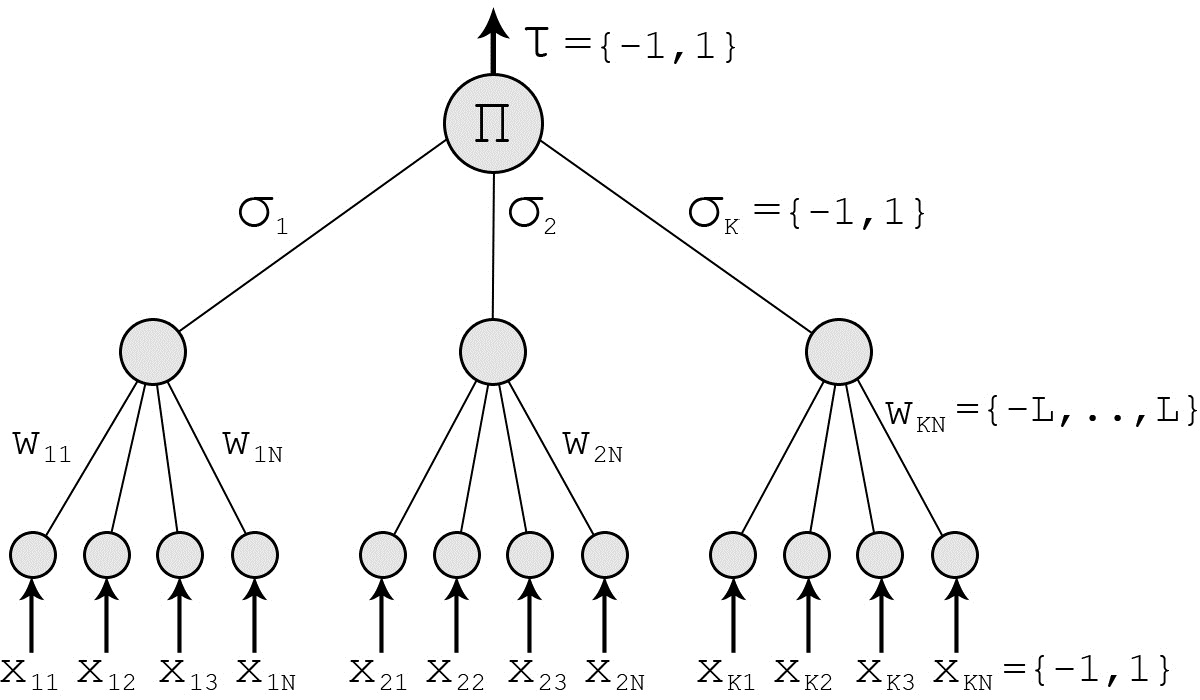
\includegraphics[width = 0.8\textwidth]{"pictures/tpm.jpg"}
\end{figure}
\end{frame}
%---------------------------------------------
\begin{frame}
\begin{itemize}
\item The two NNs participating in the communication start from private key vectors $E_k(0)$ and $D_k(0)$. Mutual learning from the exchange of public information leads the two nets to develop a common, time dependent key: $E_k(t) = - D_k(t)$. This is then used for both encryption and decryption.
\item At each step of the training process (and of encryption/decryption), a common public input vector is needed. 
\item Sender and recipient send their outputs to each other and in case they do not agree on them, weight are updated according
to a Hebbian learning rule.
\item As soon as the two NNs are synchronized, so they stay forever.
\end{itemize}
\end{frame}

%---------------------------------------------
\begin{frame}
\frametitle{KKK: Shamir's Insights}
In the paper cited before, no mathematical proof of its core principle, synchronization, is given. This result was instead attained in \cite{shamir}. Such work also contains a section dedicated to the cryptanalysis of KKK. Besides it is robust against attacks based on intercepting the key using the same neural network structure, this protocol can be broken using
\begin{itemize}
\item Genetic Attacks;
\item Geometric Attacks;
\item Probabilistic Attacks.
\end{itemize}
These results marked the beginning of a long period without any substantial contribution to neural cryptography.
\end{frame}

%------------------------------------------





%------------------------------------------------
\section{Neural Cryptanalysis}
\begin{frame}
\frametitle{Neural Cryptanalysis}
Not only NNs reveal themselves capable of learning how to communicate securely: recent studies show they can be employed
to perform efficient cryptanalysis. Consider the family of block ciphers released by NSA in \cite{nsa}, namely
\begin{itemize}
\item \textbf{Simon}, a cipher efficient in hardware implementations in IoT (Internet of Things) devices;
\item \textbf{Speck}, the sister algorithm of Simon, optimized for software implementations.
\end{itemize}
Both algorithms are compositions of the basic functions of modular addition, bitwise rotation and bitwise addition.
\end{frame}

%----------------------------------------------------------
\begin{frame}
\frametitle{Simon}
\begin{columns}[c]
\column{0.55\textwidth} 
\begin{figure}
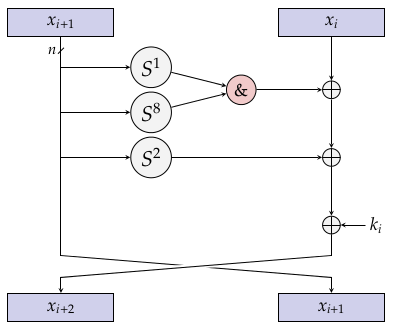
\includegraphics[width = 0.9\textwidth]{"pictures/simon.png"}
\end{figure}
\column{0.6\textwidth}
\begin{itemize}
\item The attack to Simon cipher consists in recovering the key, given a set of plaintext-ciphertext pairs.
\item MLPs are employed; input layer has one neuron per each bit of the plaintext-ciphertext pairs. Output layer has same size of the key; each cell is binary.
\item Activation function is chosen to be the Linear Rectifier:
	\begin{equation*}
	y = \sum_{j}w_j x_j + b.
	\end{equation*}
\end{itemize}
\end{columns}
\end{frame}

\begin{frame}
\frametitle{Speck}
A more advanced attack was developed against Speck, by making use of convolutional NNs to build a (neural) distinguisher. 
\begin{itemize}
\item Let $F: \{0,1\}^n \longrightarrow \{0,1\}^m$ be a map (round function). A differential transition for $F$ is a pair
$$\left(\Delta_{\text{in}},\Delta_{\text{out}} \right) \in \{0,1\}^n \times \{0,1\}^m$$
\item A differential attack uses nonrandom properties of the output of the cipher when it is being given input data with known difference distribution, i. e. $\mathbb{P}\left( \Delta_{\text{in}} \rightarrow \Delta_{\text{out}}\right)$.
\item Nets are trained to distinguish the output of Speck with given input conditions from random data.
\end{itemize} 
\end{frame}

%------------------------------------------------
\section[ANC]{Adversarial Neural Cryptography}
\begin{frame}
\frametitle{Adversarial Neural Cryptography}
Neural networks can learn to protect the secrecy of their data from other neural networks. This is the core principle of Adversarial Neural Cryptography (ANC), a revolutionary approach to cryptography invented by Google researchers in 2016. Such technique is based on\\
\begin{itemize}
\item  the problem of the secure communication between two parties, when a third participant wishes to eavesdrop on it;
\item the adversarial training of NNs representing the three participants.
\end{itemize}


\end{frame}

%-----------------------------------------------
\begin{frame}
This scenario can be summarized as follows.
\begin{itemize}
\item Alice wants to sent message $P$ to Bob. $P$ and key $K$ are the input of Alice. 
\item $K$ is also known by Bob and it is used to decipher $C$, that is the output of Alice.
\item Eve wants to eavesdrop on the communication. She knows only $C$ and tries to recover $P$.
\end{itemize}
\begin{figure}
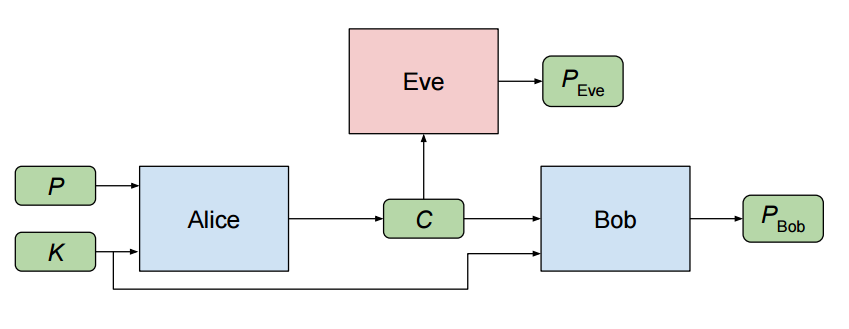
\includegraphics[width = \textwidth]{"pictures/anc.png"}
\end{figure}
\end{frame}
%---------------------------------------------------------------------------------
\begin{frame}
\frametitle{Network Architecture}
Neural Nets in the ANC share the so-called "Mix \& Transform" architecture:
\begin{itemize}
\item a first fully-connected (FC) layer, that enables mixing between input vectors;
\item a sequence of convolutional layers;
\item an output layer of a size suitable for a plaintext or a ciphertext.
\end{itemize}
Adjustment of the weights is based on Adam optimizer. The training of Eve is alternated with that of Alice and Bob.
\end{frame}
%---------------------------------------------------------------------------------
\begin{frame}
\frametitle{Chosen-Plaintext Attack ANC}
Main limitation to the security of original ANC model lies in the job of Eve, that appears to be too hard. A solution to this problem is to strengthen Eve by letting it mount a Chosen-Plaintext Attack (CPA).
\begin{figure}
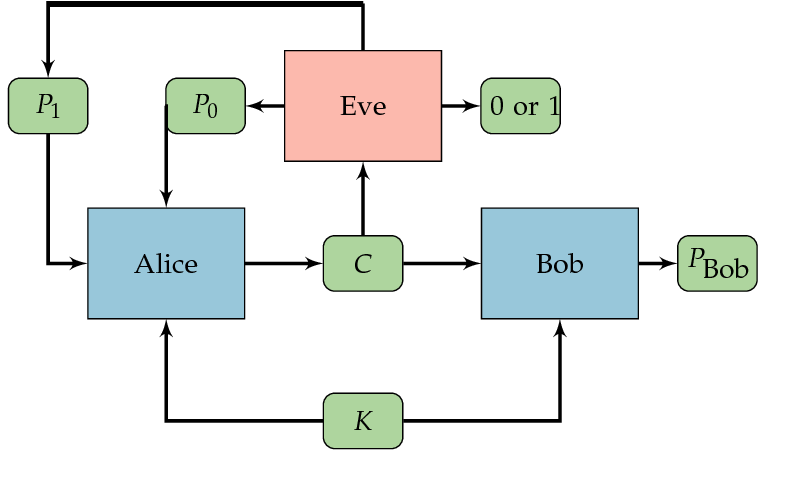
\includegraphics[width = 0.75\textwidth]{"pictures/cpa-anc.png"}
\end{figure}
\end{frame}
%---------------------------------------------------------------------------------
\begin{frame}
The resulting cryptosystem is named CPA-ANC and has the following key features.
\begin{itemize}
\item Eve choose two plaintexts $P_0$ and $P_1$ and sends them to Alice. 
\item Alice chooses one plaintext randomly, encrypts it to $C$ and send it to Bob and Eve.
\item Bob decrypts the message using its neural network.
\item Eve outputs $0$ if it believes $P_0$ was encrypted or $1$ if it believes $P_1$ was encrypted.
\end{itemize}
Training follows a similar procedure to that of the original ANC, but leads to a much stronger communication channel.
\end{frame}
%----------------------------------------------------------------------------------------
\section*{References}
\begin{frame}
\frametitle{References}
\begin{thebibliography}{99}
\bibitem[Graupe(2007)]{graupe} {\sc Graupe, D.} (2007). \textit{Principles of Artificial Neural Networks (2nd Edition)}. Word Scientific Publishing, Singapore.
 
\bibitem[McCulloch and Pitts(1943)]{mcculloch} {\sc McCulloch, W.} and {\sc Pitts, W}. (1943). \textit{A logical calculus of the ideas immanent in nervous activity}. Bulletin of Mathematical Biophysics 5, 115-133.

\bibitem[Hebb(1949)]{hebb} {\sc Hebb, D. O.} (1949). \textit{The organization of behavior; a neuropsychological theory}. Wiley, New York.

\bibitem[Rosenblatt(1958)]{rosenblatt} {\sc Rosenblatt, F.} (1958). \textit{The perceptron: A probabilistic model for information storage and organization in the brain}. Psychological Review, 65.

\bibitem[Widrow and Hoff(1960)]{widrow} {\sc Widrow, B.} and {\sc Hoff, M. E.} (1960). \textit{Adaptive Switching Circuits}. IRE WESCON Convention Record, 96-104.


\end{thebibliography}
\end{frame}
%----------------------------------------------------------------
\begin{frame}
\begin{thebibliography}{99}
\bibitem[Minsky and Papert(1969)]{minpapert} {\sc Minsky, M.} and {\sc Papert, S. A.} (1969). \textit{Perceptrons: An Introduction to Computational Geometry}. MIT Press.
\bibitem[Rumelhart, Hinton and Williams(1986)]{back} {\sc Rumelhart, D.}, {\sc Hinton, G.} and {\sc Williams, R.} (1986). \textit{Learning representations by back-propagating errors}. Nature 323, 533–536.

\bibitem[Sejnowski and Rosenberg(1987)]{sejnowski} {\sc Sejnowski, T. J.} and {\sc Rosenberg, C. R.} (1987). \textit{Parallel Networks that Learn to Pronounce English Text}. Complex Systems, 1.

\bibitem[Kingma and Ba(2015)]{adam} {\sc Kingma, D.P.} and {\sc Lei Ba, J.} (2015). \textit{Adam: a method for stochatic optimization}. CoRR.
\bibitem[Mitchell(1998)]{mit} {\sc Mitchell, M.} (1998). \textit{An introduction to Genetic Algorithms}. MIT Press.

\bibitem[Holland(1975)]{holland} {\sc Holland, J.} (1975). \textit{Adaptation in Natural and Artificial Systems}. MIT Press. 
\end{thebibliography}
\end{frame}
%--------------------------------------------------------------
\begin{frame}
\begin{thebibliography}{99}
\bibitem[Lauria(1990)]{lauria} {\sc Lauria, F. E.} (1990). \textit{On Neurocryptology.} Proceedings of the Third Italian Workshop on Parallel Architectures and Neural Networks, 337-343.

\bibitem[Volná(2000)]{volna} {\sc Volná, E.} (2000). \textit{Using Neural Network in Cryptography}. University of Ostrava.

\bibitem[Kanter, Kinzel and Kanter(2001)]{kanter} {\sc Kanter, I.}, {\sc Kinzel, W.} and {\sc Kanter, E.} (2001). \textit{Secure exchange of information by synchronization of neural networks}. Bar Ilan University.

\bibitem[Klimov, Mityagin and Shamir(2002)]{shamir} {\sc Klimov, A.}, {\sc Mityagin, A.} and {\sc Shamir, A.} (2002). \textit{Analysis of Neural Cryptography}. Weizmann Institute.


\bibitem[Abadi and Andersen(2016)]{google} {\sc Abadi, M.} and {\sc Andersen, D. G.} (2016). \textit{Learning to protect communications with Adversarial Neural Cryptography}. Google Brain

\end{thebibliography}
\end{frame}

%--------------------------------------------------------------
\begin{frame}
\begin{thebibliography}{99}
\bibitem[Coutinho et al.(2018)]{brazilians} {\sc Coutinho, M.}, {\sc Robson de Oliveira Albuquerque, R.}, {\sc Borges, F. }, {\sc Villalba, L. J. G.} and  {\sc Kim T. H.} (2018). \textit{Learning Perfectly Secure Cryptography to Protect Communications with Adversarial Neural Cryptography}. University of Brasília.

\bibitem[Jayachandiran(2018)]{jay} {\sc Jayachandiran, K.} (2018). \textit{A Machine Learning Approach for Cryptanalysis}. Rochester Institute of Technology.

\bibitem[Beaulieu et al.(2013)]{nsa} {\sc Beaulieu, R.}, {\sc Shors, D.}, {\sc Smith, J.}, {\sc Treatman-Clark, S.}, {\sc Weeks, B.} and {\sc Wingers, L.} (2013). \textit{The Simon and Speck Families of Lightweight Block Ciphers}. National Security Agency.

\bibitem[Alani(2012)]{alani} {\sc Alani, M. M.} (2012). \textit{Neuro-cryptanalysis of DES}. World Congress on Internet Security (WorldCIS-2012)

\bibitem[Gohr(2019)]{gohr} {\sc Gohr, A.} (2019). \textit{Improving Attacks on Round-Reduced Speck32/64 Using Deep Learning}. Bundesamt für Sicherheit in der Informationstechnik (BSI).

\bibitem[Shi et al.(2020)]{china} {\sc Shi, J.}, {\sc Chen, S.}, {\sc Lu, Y.}, {\sc Feng, Y.}, {\sc Shi, R.}, {\sc Yang, Y.} and {\sc Li, J.} (2020). \textit{An Approach to Cryptography Based on Continuous-Variable Quantum Neural Network}. Nature.

\end{thebibliography}
\end{frame}
\end{document} 